\section{Introduction}

Automated recognition of white blood cell morphology is often framed as a closed-set image classification task: every evaluated image is assumed to belong to one of the cell types observed during training. Under that framing, modern convolutional classifiers can achieve strong performance on curated single-cell microscopy datasets. This is scientifically useful, but it does not answer a harder operational question. A system trained to distinguish a fixed set of mature leukocyte morphologies may encounter immature, atypical, rare, or otherwise out-of-taxonomy morphologies at test time. In that setting, assigning every input to the closest known class can be misleading as an evaluation behavior, even for research-only systems.

This study investigates open-set recognition for hematological cell morphology. We define the known taxonomy as five mature leukocyte classes: basophil, eosinophil, lymphocyte, monocyte, and segmented neutrophil. All other evaluated morphologies are treated as unknown only in the protocol sense: they are outside the known training taxonomy. This terminology is deliberately narrow. An unknown sample is not a cancer label, leukemia label, malignancy label, diagnostic label, or clinically positive label. The task is not to diagnose disease. The task is to ask whether a classifier trained on a known morphology taxonomy can detect that a test image should not be forced into that taxonomy.

The distinction matters because closed-set classification and unknown rejection measure different behavior. A model may learn a compact representation for the known classes and still place an unseen but morphologically related cell close to a known class. For example, a band neutrophil may be visually and semantically close to segmented neutrophils, and lymphoid-like unknowns may be attracted toward the known lymphocyte class. Such behavior can leave closed-set accuracy high while open-set reliability remains limited. The scientific question is therefore not whether deep networks can classify known leukocytes, but whether the confidence and embedding structure of those networks support reliable rejection of unseen morphologies.

We approach this question as a reproducible evaluation study rather than as a claim of a new superior method. The internal dataset is MLL23, a large expert-annotated single-cell peripheral blood dataset with 18 morphology classes \cite{mll23_nature_2025,mll23_zenodo_2024}. We use five mature leukocyte classes as the known training taxonomy and hold the remaining classes out for open-set testing. We evaluate two split protocols: the original deterministic split and a conservative near-duplicate-aware sensitivity split. Because reliable patient or acquisition-group identifiers are not available in the working MLL23 manifests, the conservative split should be interpreted as a leakage sensitivity analysis rather than as proof of patient-level separation.

The external dataset is AML-Cytomorphology\_LMU, an independent TCIA collection of 18,365 expert-labeled single-cell images \cite{aml_lmu_tcia_2019}. We map only exact source labels to the five known classes and keep immature or atypical morphologies outside the known taxonomy. The external dataset is used only for testing. There is no external fine-tuning, external threshold calibration, external ViM fitting, external model selection, or taxonomy modification. This makes AML-LMU central to the paper: it evaluates whether conclusions drawn internally survive a change in acquisition domain and class composition.

The experiments cover three families of approaches. First, we evaluate a conventional ImageNet-pretrained ResNet18 classifier with post-hoc open-set scores, including maximum softmax probability (MSP), energy, distance-based scores, ReAct, and ViM. Second, we evaluate representation-learning alternatives, including supervised contrastive learning and ArcFace-style angular-margin training. Third, we evaluate persistent homology in two distinct roles. Cubical persistent homology over image, morphology-candidate, and feature-map filtrations is treated as a predictive ablation. Vietoris-Rips persistent homology over learned embedding clouds is treated only as an explanatory analysis of representation topology. These roles are intentionally separated, because using topology as a classifier feature is a different claim from using topology to describe learned geometry.

The central finding is conservative but important: strong known-class classification does not imply reliable open-set recognition of unseen hematological morphologies. Across internal five-seed experiments, closed-set macro-F1 remained near 0.97, yet open-set metrics were more variable and morphology dependent. ArcFace improved some known-class geometry summaries and showed promising behavior in selected conditions, but it failed multiseed and split confirmation as a robust superior representation. Under external AML-LMU validation, every principal system degraded substantially, and the internal ranking of post-hoc open-set methods did not transfer cleanly. In particular, CE+ViM was the stable internal baseline, but MSP outperformed ViM externally in the principal blocks.

Our contribution is therefore a claim-disciplined evaluation framework and evidence base for open-set hematological morphology recognition under representation instability and acquisition-domain shift. The paper makes the following contributions:
\begin{itemize}
\item We construct a reproducible open-set evaluation protocol for hematological cell morphology, with explicit known and unknown taxonomies, strict train/validation/test separation, and frozen rules for unknown terminology.
\item We perform multiseed and split-sensitivity analysis of post-hoc open-set scoring and representation learning, showing that closed-set geometry improvements do not automatically translate into robust unknown rejection.
\item We externally evaluate frozen systems on AML-LMU without external training or tuning, showing substantial domain-shift degradation and changed method rankings.
\item We analyze morphology-dependent failure modes using per-class open-set metrics, known-class attractors, embedding geometry, and secondary Vietoris-Rips topology.
\end{itemize}

\begin{figure}[htbp]
\centering
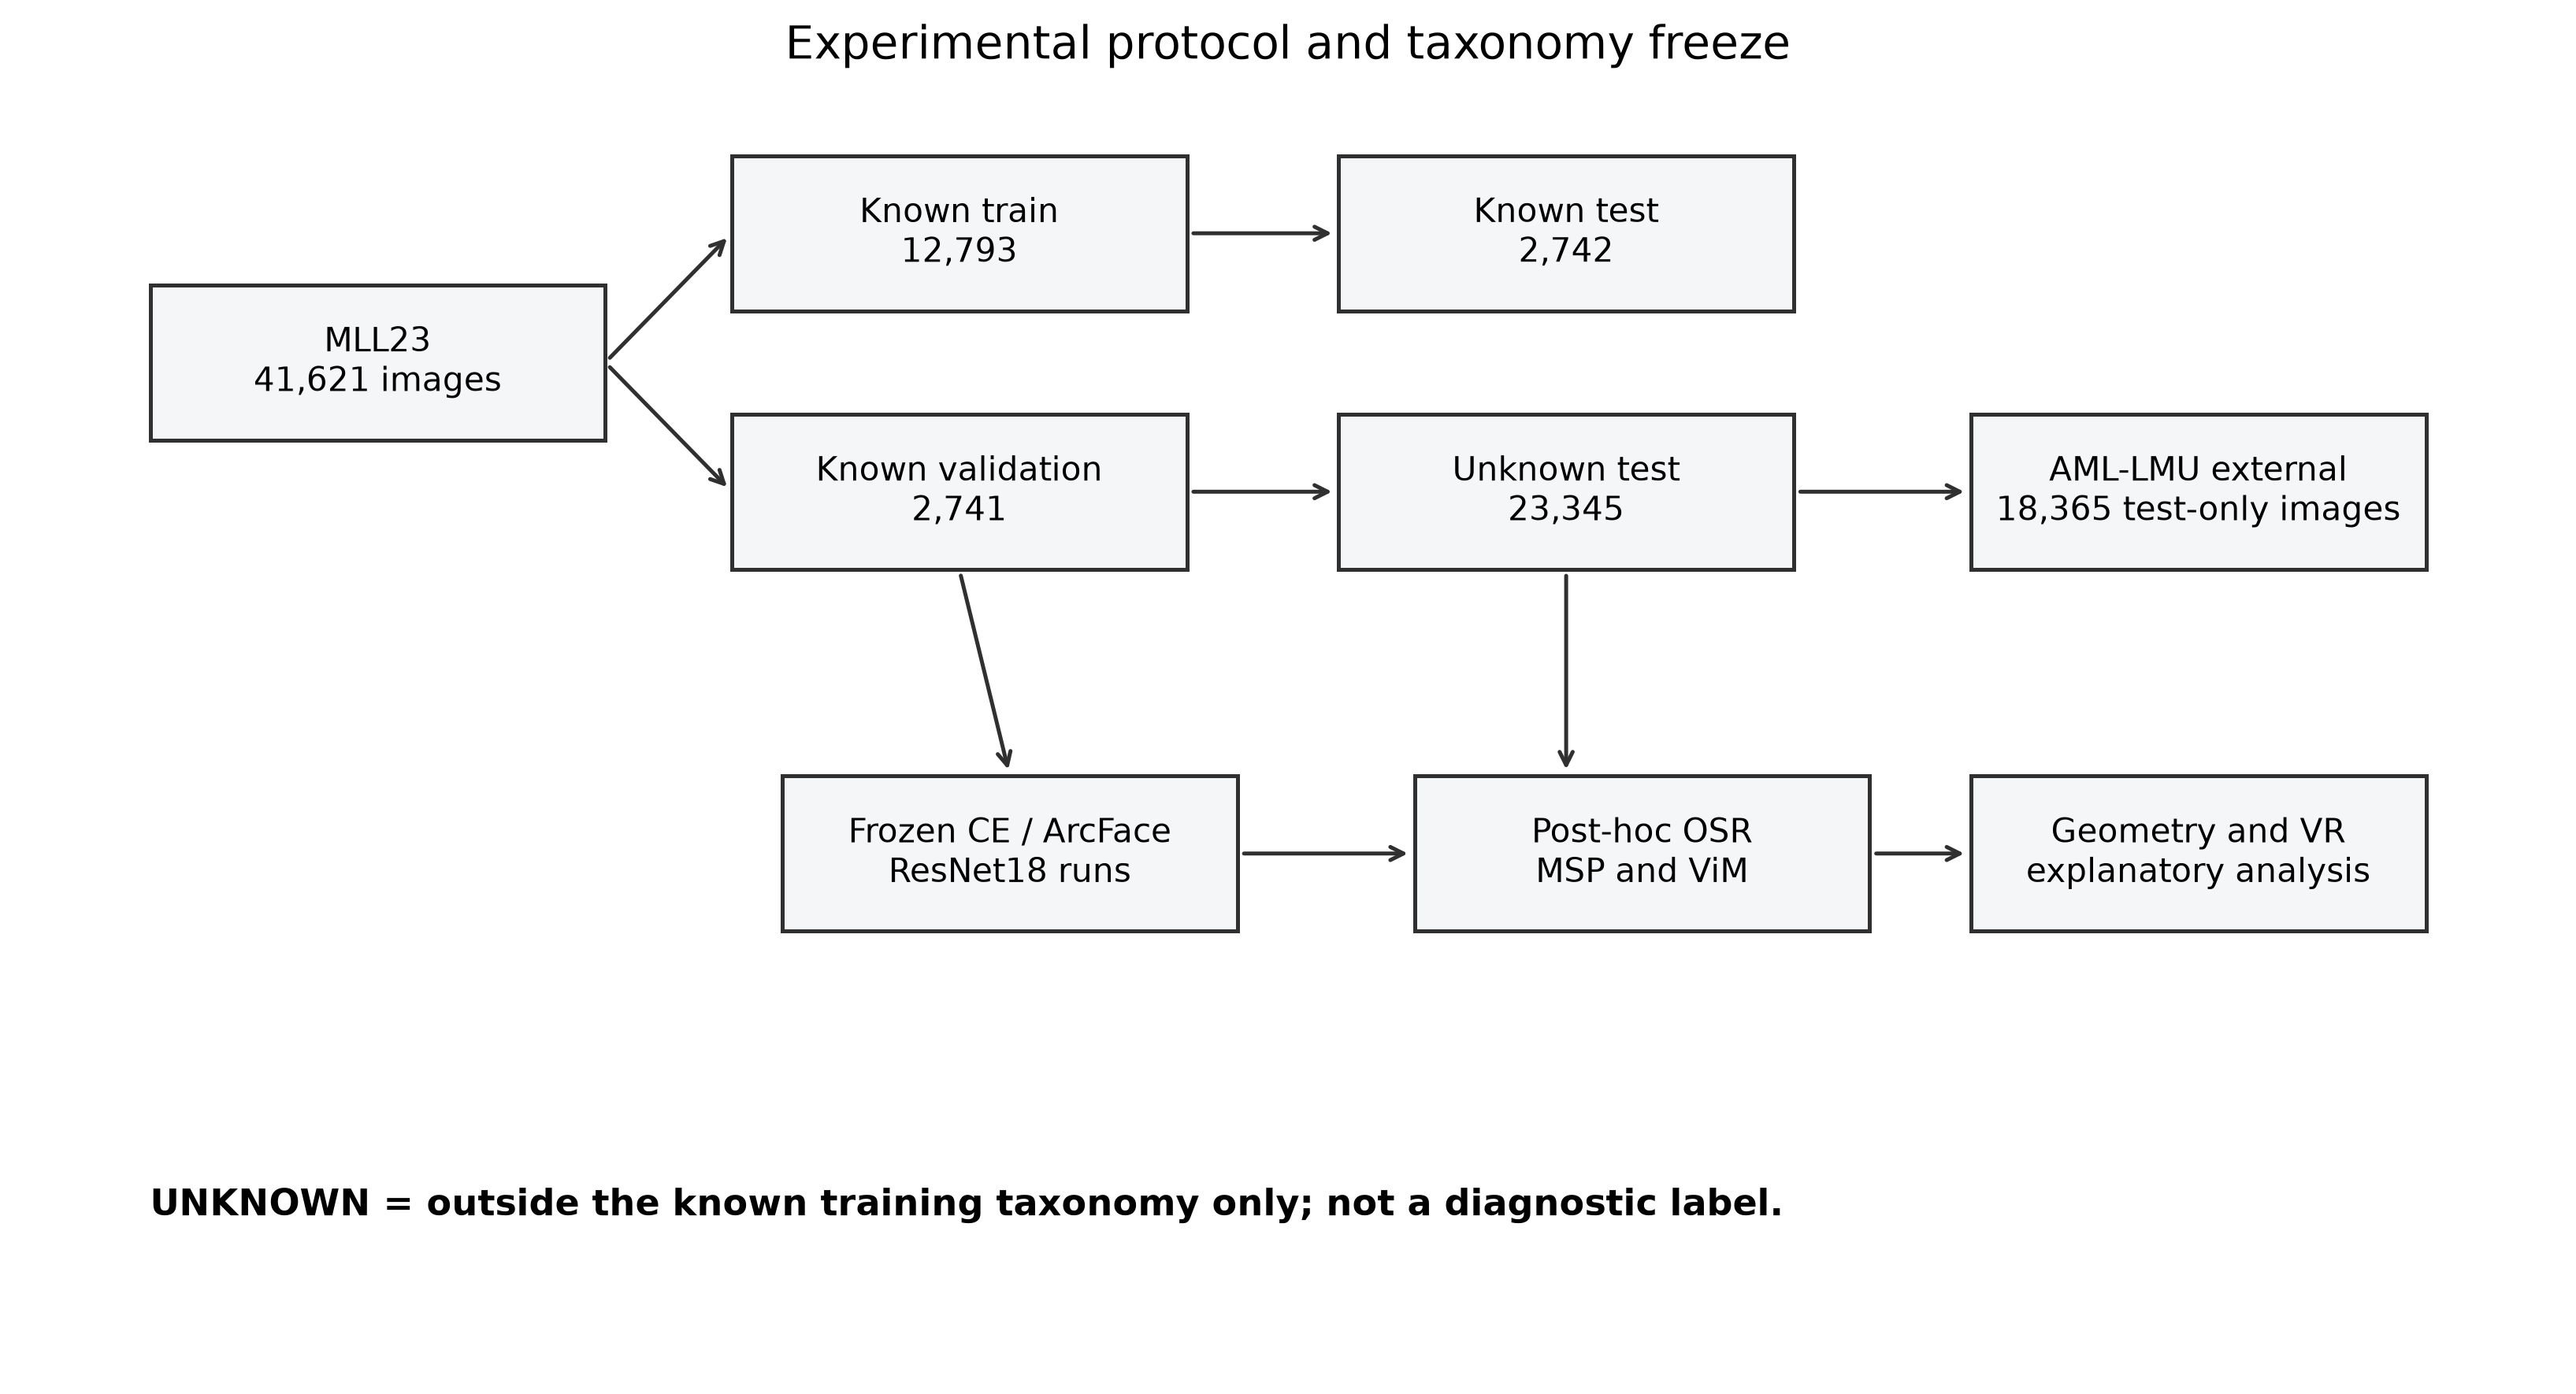
\includegraphics[width=\textwidth]{figures/figure1_protocol.png}
\caption{Frozen open-set evaluation protocol. MLL23 supports internal multiseed and split-sensitivity analysis; AML-LMU is used as an external test-only domain.}
\label{fig:protocol}
\end{figure}
